%% LyX 2.4.4 created this file.  For more info, see https://www.lyx.org/.
%% Do not edit unless you really know what you are doing.
\documentclass[english]{article}
\usepackage[T1]{fontenc}
\usepackage[latin9]{inputenc}
\usepackage{units}
\usepackage{enumitem}
\usepackage{amsmath}
\usepackage{amsthm}
\usepackage{cancel}
\usepackage{geometry}
\geometry{verbose,tmargin=1in,bmargin=1in,lmargin=1in,rmargin=1in}

\makeatletter

%%%%%%%%%%%%%%%%%%%%%%%%%%%%%% LyX specific LaTeX commands.
%% Because html converters don't know tabularnewline
\providecommand{\tabularnewline}{\\}

%%%%%%%%%%%%%%%%%%%%%%%%%%%%%% Textclass specific LaTeX commands.
\numberwithin{equation}{section}
\numberwithin{figure}{section}
\newlength{\lyxlabelwidth}      % auxiliary length 

%%%%%%%%%%%%%%%%%%%%%%%%%%%%%% User specified LaTeX commands.
\usepackage{hyperref}
\usepackage[usenames,dvipsnames,table]{xcolor} %adds additional color options
\hypersetup{colorlinks=true, urlcolor=black}

\usepackage{fancyhdr}
\usepackage{lastpage}
\pagestyle{fancy}
\usepackage{enumitem}
\usepackage{ifthen}
%sets math fonts to be more readable
\everymath=\expandafter{\the\everymath\displaystyle}
%\DeclareMathSizes{10}{10}{10}{10}
\usepackage{multicol}

\usepackage{tikz}
\usetikzlibrary{plotmarks}
\usepackage{pgfplots}
\pgfplotsset{compat=newest}

\usepackage{calc}
\usepackage[nomessages]{fp}

\usepackage{advdate}    % Advancing/saving dates
\usepackage{datetime}   % Dates formatting
\usepackage{datenumber} % Counters for dates

\usepackage{fancybox} %%ovalbox and fancy box settings

\usepackage[super]{nth} %easy 1st, 2nd, etc

\usepackage{forest} %%for tree diagram
% Added by lyx2lyx
\setlength{\parskip}{\smallskipamount}
\setlength{\parindent}{0pt}

\makeatother

\usepackage{babel}
\begin{document}
\renewcommand{\author}{Dr.\,James Ashe}

\newcommand{\classNum}{107}

\newcommand{\classSec}{7 and 10}

\newcommand{\nameType}{}

\newcommand{\examType}{Exam 3 Review}

\renewcommand{\date}{Exam 3 is on the\formatdate{27}{10}{2014}}

%%First page's header%%%%%%%%%%%%%%%%%%%%%%
\fancypagestyle{firststyle} %%header settings for first pagr
{
	\fancyhead[L]{MTH \classNum{}(\classSec{}) \author{}\\
	\textbf{\examType{}} \date{}}
	\fancyhead[C]{\textbf{\nameType}}
	\setlength{\headsep}{14pt}
}
%%%%%%%%%%%%%%%%%%%%%%%%%%%%%%%%%%%%%%%%%%

%%Next page's header%%%%%%%%%%%%%%%%%%%%%%%
%\setlist{nolistsep}
\lhead{MTH \classNum{}(\classSec{})} 
\chead{\textbf{\nameType}} 
\cfoot{\thepage{}~of~\pageref{LastPage}} 
\setlength{\headsep}{5pt} 
%%%%%%%%%%%%%%%%%%%%%%%%%%%%%%%%%%%%%%%%%%%

%%Various settings; see the preamble for other settings%%%%%
%%\setenumerate[0]{leftmargin=12pt,itemindent=0pt,labelwidth=0pt}
%\setlist[2]{noitemsep}
%\setlist{nosep}
\setlist{itemsep=-3pt,topsep=-2pt}
\renewcommand{\labelenumi}{\textbf{\arabic{enumi}.}}
\renewcommand{\labelenumii}{\textbf{\alph{enumii}.}}
\thispagestyle{firststyle}
%%%%%%%%%%%%%%%%%%%%%%%%%%%%%%%%%%%%%%%%%%
\newcommand{\xmax}{10}
\newcommand{\xmin}{-10}
\newcommand{\xstep}{0} %must be xmin+n
\newcommand{\ymax}{10}
\newcommand{\ymin}{-10}
\newcommand{\ystep}{0} %must be ymin+n

\newcommand{\xspace}{\hspace*{40pt}}
\newcommand{\yspace}{\vspace*{.25cm}}
\newcommand{\rowColor}{gray!35}
\large
\begin{enumerate}[resume]
\item A card is dealt from a well-shuffled, standard deck of $52$ cards.
Find the probability of being dealt each of the following.\begin{multicols}{2}

\begin{enumerate}
\item A red card

\begin{enumerate}
\item []$\frac{n(\mbox{red cards})}{n(\mbox{cards})}=\frac{26}{52}=\frac{1}{2}$\yspace
\end{enumerate}
\item A queen

\begin{enumerate}
\item []$\frac{n(\mbox{queens})}{n(\mbox{cards})}=\frac{4}{52}=\frac{1}{13}$\yspace
\end{enumerate}
\item A club

\begin{enumerate}
\item []$\frac{n(\mbox{clubs})}{n(\mbox{cards})}=\frac{13}{52}=\frac{1}{4}$\yspace\columnbreak
\end{enumerate}
\item The queen of clubs

\begin{enumerate}
\item []$\frac{n(\mbox{queen of clubs})}{n(\mbox{cards})}=\frac{1}{52}$\yspace
\end{enumerate}
\item A queen or a club

\begin{enumerate}
\item []$\frac{n(\mbox{queens or clubs})}{n(\mbox{cards})}=\frac{4+13-1}{52}=\frac{16}{52}=\frac{4}{13}$\yspace
\end{enumerate}
\item not a queen

\begin{enumerate}
\item []$1-\frac{4}{52}=\frac{48}{52}=\frac{12}{13}$\yspace
\end{enumerate}
\end{enumerate}
\end{multicols}\vfill
\item Three coins are tossed. Find each of the following:\begin{multicols}{2}

\begin{enumerate}
\item the sample space\\
\forestset{  
	L1/.style={rectangle, rounded corners, very     thick},   	
	L2/.style={rectangle, rounded corners, very     thick,
		edge={black,line width=.75pt,line cap=round}},   	
	L3/.style={rectangle, rounded corners, very     thick,
		edge={black,line width=.75pt,line cap=round}},   	
	L4/.style={rectangle, rounded corners, very     thick,
	edge={black,line width=.75pt,line cap=round}}, 
}

\begin{forest}     
	for tree={
		scale=.75,        
		grow=0,
		reversed, %tree direction         
		parent anchor=east,
		child anchor=west, %edge anchors   		edge={line cap=round},
		outer sep=+1pt, %edge/node connection  		rounded corners,
		%minimum width=15mm,
		%minimum height=8mm, %node shape         l 		sep=10mm %level distance     
		}   
[Start,L1
	[H,L2         
		[H,L3            
			[H \{HHH\},L4] 
			[T \{HHT\},L4]         
		]         
		[T,L3          
			[H \{HTH\},L4]
			[T \{HTT\},L4]
		]               
	]
	[T,L2         
		[H,L3            
			[H \{THH\},L4,]
			[T \{THT\},L4,]         
		]         
		[T,L3          
			[H \{TTH\},L4]
			[T \{TTT\},L4]
		]               
	]  
] 
\end{forest}\yspace\columnbreak
\item the event, $E_{1}$, that exactly two are tails

\begin{enumerate}
\item []$E_{1}=\{HTT,THT,TTH\}$\yspace
\end{enumerate}
\item the event, $E_{2}$, that at least two are tails.

\begin{enumerate}
\item []$E_{2}=\{HTT,THT,TTH,TTT\}$\yspace
\end{enumerate}
\item the probability and odds of $E_{1}$

\begin{enumerate}
\item []$p(E_{1})=\frac{3}{8}$\yspace
\item []$o(E_{1})=3:5$\yspace
\end{enumerate}
\item the probability and odds of $E_{2}$

\begin{enumerate}
\item []$p(E_{2})=\frac{4}{8}=\frac{1}{2}$\yspace
\item []$o(E_{2})=1:1$\yspace
\end{enumerate}
\end{enumerate}
\end{multicols}\vfill
\item Five cards are dealt (without replacement) from a well-shuffled standard
deck. \textbf{Just write the formula }for the probability of the following:\begin{multicols}{2}

\begin{enumerate}
\item being dealt $5$ spades

\begin{enumerate}
\item []$\frac{_{13}C_{5}}{_{52}C_{5}}$\yspace
\end{enumerate}
\item being dealt $4$ spades and $1$ heart

\begin{enumerate}
\item []$\frac{_{13}C_{4}\cdot_{13}C_{1}}{_{52}C_{5}}=\frac{_{13}C_{4}\cdot13}{_{52}C_{5}}$\yspace
\end{enumerate}
\item being dealt all the same suit.

\begin{enumerate}
\item []$\frac{_{4}C_{1}\cdot_{13}C_{5}}{_{52}C_{5}}=\frac{4\cdot_{13}C_{5}}{_{52}C_{5}}$\yspace
\end{enumerate}
\item not being dealt all the same suit.

\begin{enumerate}
\item []$1-$$\frac{4\cdot_{13}C_{5}}{_{52}C_{5}}$\yspace
\end{enumerate}
\end{enumerate}
\end{multicols}\vfill\newpage
\item A drawer has $7$ socks. $4$ socks are black and $3$ are white socks.
John randomly pulls out $4$ socks. Find the probability of the following:\begin{multicols}{2}

\begin{enumerate}
\item all $4$ socks are black.

\begin{enumerate}
\item []$\frac{_{4}C_{4}}{_{7}C_{4}}=\frac{1}{35}$\yspace
\end{enumerate}
\item exactly $2$ are white.

\begin{enumerate}
\item []$\frac{_{3}C_{2}\cdot_{4}C_{2}}{_{7}C_{4}}=\frac{3\cdot6}{35}=\frac{18}{35}$\yspace
\item []$2$ are white and $2$ are black
\end{enumerate}
\columnbreak
\item at least $3$ are white.

\begin{enumerate}
\item []$\frac{_{3}C_{3}\cdot_{4}C_{0}+_{3}C_{4}\cdot_{4}C_{0}}{_{7}C_{4}}=\frac{1\cdot1+0\cdot1}{35}=\frac{1}{35}$\yspace
\item []$3$ OR $4$ are white
\end{enumerate}
\item at most $2$ are black. 

\begin{enumerate}
\item []$\frac{_{4}C_{0}\cdot_{3}C_{4}+_{4}C_{1}\cdot_{3}C_{3}+_{4}C_{2}\cdot_{3}C_{2}}{_{7}C_{4}}=\frac{1\cdot0+4\cdot1+6\cdot3}{35}=\frac{22}{35}$\yspace
\item []$0$ or $1$ or $2$ are black.
\end{enumerate}
\end{enumerate}
\end{multicols}
\begin{itemize}
\item Note: Above, $_{3}C_{4}=0$ as there are $0$ ways to choose $4$
white socks if there are only $3$. I will \textbf{not} have a situation
like this on the exam.\yspace\vfill
\end{itemize}
\item Gregor's Garden Corner buys $40\%$ of its plants from the Green Growery
and the rest from Herb's Herbs. Of the plants from the Green Growery,
$20\%$ must be returned, and $10\%$ of those from Herb's Herbs must
be returned. \begin{multicols}{2}

\begin{enumerate}
\item draw a tree diagram describing the probability\\
\tikzset{abovelabel/.style={midway,above,font=\scriptsize}} 
\tikzset{belowlabel/.style={midway,below,font=\scriptsize}} 

\forestset{  
	L1/.style={rectangle, rounded corners, very     thick},   	
	L2/.style={rectangle, rounded corners, very     thick,
		edge={black,line width=.75pt,line cap=round}},   	
	L3/.style={rectangle, rounded corners, very     thick,
		edge={black,line width=.75pt,line cap=round}},   	
	L4/.style={rectangle, rounded corners, very     thick,
	edge={black,line width=.75pt,line cap=round}}, 
}

\begin{forest}     
	for tree={
		scale=1,        
		grow=0,
		reversed, %tree direction         
		parent anchor=east,
		child anchor=west, %edge anchors   		edge={line cap=round},
		outer sep=+1pt, 
		%edge/node connection rounded corners,
		%minimum width=15mm,
		%minimum height=8mm, 
		%node shape
		l sep=1.5cm    
		}   
[Start,L1
	[G,edge label={node[abovelabel]{$.40$}},L2
		[R, edge label={node[abovelabel]{$.20$}}, L3]         
		[R',edge label={node[belowlabel]{$.80$}}, L3]               
	]
	[H,edge label={node[belowlabel]{$.60$}},L2
		[R, edge label={node[abovelabel]{$.10$}}, L3]        
		[R',edge label={node[belowlabel]{$.90$}}, L3]                
	]  
] 
\end{forest}\yspace\vfill\columnbreak
\item find the probability that a plant must be returned and it is from
Herb's Herbs.

\begin{enumerate}
\item []$p(H\cap R)=(.60)(.10)=.06$\yspace
\end{enumerate}
\item find the probability that a plant from the Green Growery must be returned.

\begin{enumerate}
\item []$p(R\mid G)=.20$\yspace
\end{enumerate}
\item find the probability that a plant must be returned. 

\begin{enumerate}
\item []A returned plant can be from Herb's OR Gregory, \\
$p(R)=p(H\cap R)+p(G\cap R)=(.6)(.1)+(.4)(.2)=.06+.08=.14$\yspace
\end{enumerate}
\end{enumerate}
\end{multicols}\vfill
\item Use the provided table to answer the following questions.

\begin{tabular}{|c|c|c|c|}
\hline 
\textbf{Age} & \textbf{Obama} & \textbf{McCain} & \textbf{Other/NA}\tabularnewline
\hline 
18-29 & 11.9\% & 5.8\% & 0.4\%\tabularnewline
\hline 
30-44 & 15.1\% & 13.3\% & 0.6\%\tabularnewline
\hline 
45-64 & 18.5\% & 18.1\% & 0.4\%\tabularnewline
\hline 
65+ & 7.2\% & 8.5\% & 0.3\%\tabularnewline
\hline 
\end{tabular}
\begin{enumerate}
\item What is the probability that a voter under $45$ voted for McCain.

\begin{enumerate}
\item []$p(M\mid\mbox{under }45)=\frac{n(M\cap\mbox{under }45)}{n(\mbox{under }45)}=\frac{.058+.133}{.119+.058+.004+.151+.133+.006}=\frac{.191}{.471}\approx40.55\%$\yspace
\end{enumerate}
\item What is the probability that a person who voted for McCain is $45$
or older.

\begin{enumerate}
\item []$p(\mbox{over }45\mid M)=\frac{n(\mbox{over }45\cap M)}{n(M)}=\frac{.181+.085}{.058+.133+.181+.085}=\frac{.266}{.457}\approx58.21\%$\yspace
\end{enumerate}
\end{enumerate}
\vfill
\item MHU is holding a raffle to raise money for a new internet service.
The tickets cost $\$10$ each. The value and number of each prize
to be given away is listed in the provided table. Find the expected
value of a ticket under the given circumstances. 

\begin{tabular}{|c|c|c|}
\hline 
\textbf{Prize} & \textbf{Value} & \textbf{\# }\tabularnewline
\hline 
Vacation & $\$3,000$ & 1\tabularnewline
\hline 
Stereo & $\$500$ & 5\tabularnewline
\hline 
Books & $\$100$ & 10\tabularnewline
\hline 
T-shirt & $\$20$ & 100\tabularnewline
\hline 
\end{tabular}
\begin{enumerate}
\item $200$ tickets

\begin{enumerate}
\item []There are $200-116=84$ losing tickets.\\
$EV=2990(\frac{1}{200})+490(\frac{5}{200})+90(\frac{10}{200})+10(\frac{100}{200})-10(\frac{84}{200})$\\
\hspace{0cm}\hphantom{$EV$}$=\$32.5$\yspace
\end{enumerate}
\item $1000$ tickets

\begin{enumerate}
\item []There are $1000-116=884$ losing tickets.\\
$EV=2990(\frac{1}{1000})+490(\frac{5}{1000})+90(\frac{10}{1000})+10(\frac{100}{1000})-10(\frac{884}{1000})$\\
\hspace{0cm}\hphantom{$EV$}$=-\$1.5$\yspace
\end{enumerate}
\end{enumerate}
\item Of all the flashlights is a large shipment, $15\%$ have a defective
bulb, $10\%$ have a defective battery, and $5\%$ have both defects.
If you buy one of these flashlights, find the probability of the following:\begin{multicols}{2}

\begin{enumerate}
\item a defective bulb or a defective battery

\begin{enumerate}
\item []$p(Batt'\cup Bulb')=.10+.05+.05$
\item []\hspace{0cm}\hphantom{[$p(Batt'\cup Bulb')$}$=.20$\yspace
\end{enumerate}
\item a good bulb or a good battery

\begin{enumerate}
\item []$p((Batt'\cap Bulb'))=1-.05=.95$\yspace
\end{enumerate}
\item a defective bulb and a defective battery. 

\begin{enumerate}
\item []$p(Bulb'\cap Batt')=.05$\yspace
\end{enumerate}
\item just a defective bulb

\begin{enumerate}
\item []$p(Bulb'-Batt')=.10-.05=.05$\yspace\columnbreak
\end{enumerate}
\end{enumerate}
%%%% M or A %%%%%
\begin{center}
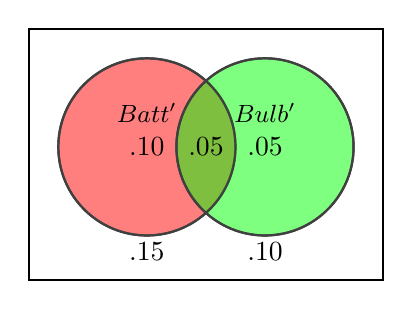
\begin{tikzpicture}[scale=.75]
	\def\circleA{(0,0) circle (1.5)} %A
	\def\circleB{(0:2) circle (1.5)} %B

	\colorlet{circle edgeA}{black!75} 
	\colorlet{circle areaA}{red!100}
	\colorlet{circle edgeB}{black!75} 
	\colorlet{circle areaB}{green!100}

	\tikzset{
		filledA/.style={fill=circle areaA, draw=circle edgeA, thick},
		filledB/.style={fill=circle areaB, draw=circle edgeB, thick},
		outlineA/.style={draw=circle edgeA, thick},
		outlineB/.style={draw=circle edgeB, thick},
	}
	
	\begin{scope}[fill opacity=0.5]         
			\fill[filledA] \circleA;
			\fill[filledB] \circleB;    
	\end{scope}

	\draw[outlineA] \circleA node[above=5pt] {\small $Batt'$} node[] { $.10$} node[below=-1pt] at (0,-1.5) {$.15$}; 
	\draw[outlineB] \circleB node[above=5pt] {\small $Bulb'$} node[] { $.05$} node[below=-1pt] at (2,-1.5) { $.10$};
	\draw (1,0) node {.05};
	\draw[thick] (-2,-2.25) rectangle (4,2) node[anchor=south east] at (current bounding box.south east) {$$}; 
\end{tikzpicture}
\end{center}

\end{multicols}\vfill\newpage
\item A single card is dealt from a well-shuffled standard deck. The probability
of being dealt a jack is $\nicefrac{4}{52}$, and the probability
of being dealt a red card is $\nicefrac{1}{2}$. 

\begin{enumerate}
\item Are the events ``being dealt a jack'' and ``being dealt a red card''
independent?

\begin{enumerate}
\item []$p(J)=\frac{4}{52}=\frac{1}{13}$ and $p(J\mid R)=\frac{n(J\cap R)}{n(R)}=\frac{2}{26}=\frac{1}{13}$\yspace
\item []So yes they are indepedent since $p(J)=p(J\mid R)$.\yspace
\end{enumerate}
\item Are the events ``being dealt a jack'' and ``being dealt a red card''
mutually exclusive? 

\begin{enumerate}
\item []$J\cap R\neq\emptyset$, since there is a red jack (the jack of
hearts and the jack of diamonds).
\item []So they are not mutually exclusive.\yspace
\end{enumerate}
\item Are the events ``being dealt a jack'' and ``being dealt a queen''
mutually exclusive?

\begin{enumerate}
\item []$J\cap Q=\emptyset$, since a card cannot be both a queen and jack.
\item []So they are mutually exclusive.\yspace
\end{enumerate}
\item Suppose instead that a card is dealt, replaced, and then another card
is dealt. Are the events ``being dealt a jack \nth{1}'' and ``being
dealt a queen \nth{2} independent? are they mutually exclusive?

\begin{enumerate}
\item []Yes they are independent. Since the card was replaced and reshuffled,
the \nth{1} draw does not affect the probability of the \nth{2}
draw. They are not mutually exclusive because you can get a Jack and
then a Queen.\yspace
\end{enumerate}
\end{enumerate}
\item A fair six-sided dice is rolled 5 times. Find the probability of the
following:

\begin{enumerate}
\item All $2$'s are rolled.

\begin{enumerate}
\item []$p(\mbox{five }2's)=\frac{1}{6}\cdot\frac{1}{6}\cdot\frac{1}{6}\cdot\frac{1}{6}\cdot\frac{1}{6}=\frac{1}{6^{5}}$\yspace
\end{enumerate}
\item Four $2$'s are rolled and the \nth{5} roll is a $1$.

\begin{enumerate}
\item []$p(\mbox{four }2's\cap\mbox{one }1)=(\frac{1}{6}\cdot\frac{1}{6}\cdot\frac{1}{6}\cdot\frac{1}{6})\cdot\frac{1}{6}=\frac{1}{6^{5}}$\yspace\vfill
\end{enumerate}
\end{enumerate}
\end{enumerate}

\end{document}
